\section{Sztuczna inteligencja (Bartosz Strzelecki)}
Nawigacja przeciwników została zrealizowana poprzez wbudowany w silnik Unity system NavMesh. Pozwala nam on na łatwe wyznaczenie powierzchni, po której mogą poruszać
się postacie niekontrolowane przez gracza oraz realizuję zadanie wyznaczania ścieżki dla tych postaci.

\begin{figure}[h]
\centering
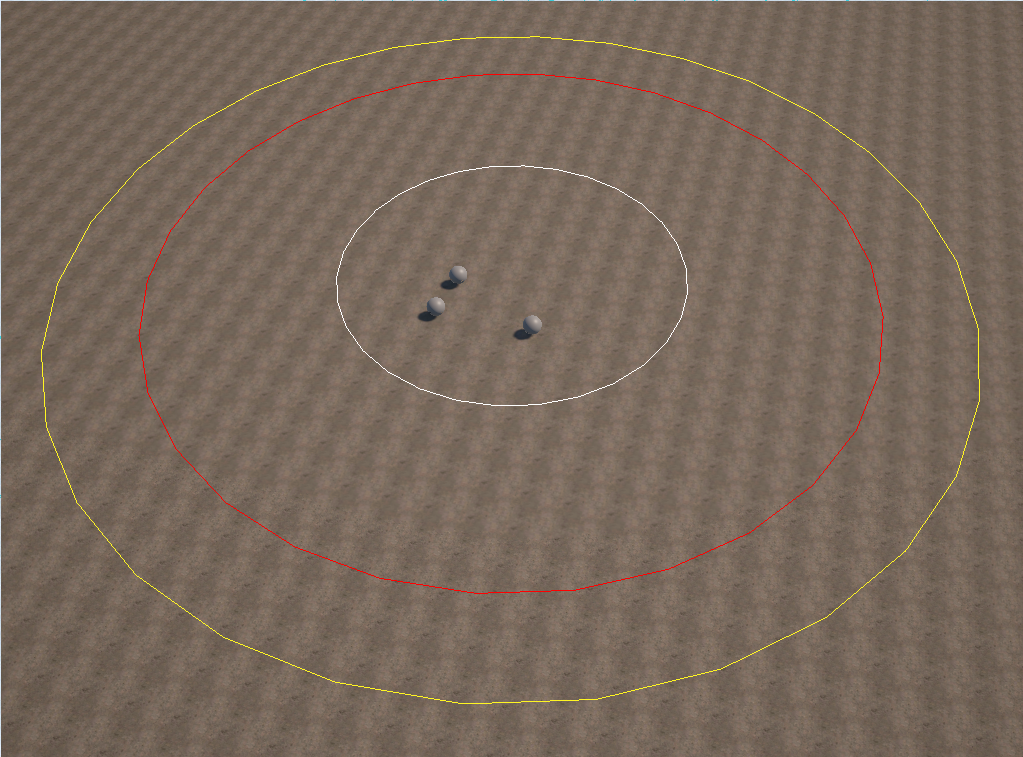
\includegraphics[width=0.6\textwidth]{images/ai}
\caption{Obraz przedstawia zasięgi odpowiednich regionów.}
\label{fig:regions}
\end{figure}

Przeciwnicy są kontrolowani poprzez jeden obiekt przydzielający cele każdemu przypisanemu wrogowi. W normalnym trybie wrogowie poruszają się w sposób losowy
w obrębie wyznaczonej przestrzeni (biały okrąg). Kiedy przyjazne jednostki znajdą się w wystarczającej odległości (czerwony okrąg), przeciwnicy obiorą sobie za cel jedną z nich.
Po opuszczeniu przez drużynę gracza wyznaczonego obszaru (żółty okrąg) wrogowie wracają do poruszania się w sposób losowy w obrębie białego okręgu.
